%%%%%%%%%%%%%%%%%%%%%%%%%%%%%%%%%%%%%%%%%
% Beamer Presentation
% LaTeX Template
% Version 1.0 (10/11/12)
%
% This template has been downloaded from:
% http://www.LaTeXTemplates.com
%
% License:
% CC BY-NC-SA 3.0 (http://creativecommons.org/licenses/by-nc-sa/3.0/)
%
%%%%%%%%%%%%%%%%%%%%%%%%%%%%%%%%%%%%%%%%%

%----------------------------------------------------------------------------------------
%	PACKAGES AND THEMES
%----------------------------------------------------------------------------------------

\documentclass{beamer}
\usepackage{xcolor}
\usepackage{graphicx}
\usepackage{tikz}
\usepackage{listings}
\usepackage{multicol}

\definecolor{applegreen}{rgb}{0.55, 0.71, 0.0}
\definecolor{blue(ncs)}{rgb}{0.0, 0.45, 0.60}
\definecolor{burgundy}{rgb}{0.5, 0.0, 0.13}

\definecolor{cadet}{rgb}{0.33, 0.41, 0.47}
\definecolor{airforceblue}{rgb}{0.36, 0.54, 0.66}

\lstdefinestyle{C}{
  language=C,
  emptylines=1,
  breaklines=true,
  basicstyle=\ttfamily\color{black},
  identifierstyle=\ttfamily,
  keywordstyle=\color[rgb]{0.0, 0.0, 1.0},
  stringstyle=\color[rgb]{1.0, 0.0, 0.0},
  commentstyle=\color{gray}\slshape,
}

\lstdefinestyle{assembly}{
  emptylines=1,
  breaklines=true,
  basicstyle=\ttfamily\color{black},
  identifierstyle=\ttfamily,
  keywordstyle=\color[rgb]{1.0, 0.0, 1.0},
  stringstyle=\color[rgb]{1.0, 0.0, 0.0},
  commentstyle=\color{gray}\slshape,
  morekeywords={vmovapd, vfmadd231pd,vfnmadd213pd, vmulpd},
}

\lstdefinestyle{qfunc}{
  language=C,
  emptylines=1,
  breaklines=true,
  basicstyle=\ttfamily\color{black},
  commentstyle=\color{gray}\slshape,
  moredelim=**[is][\color{applegreen}]{@}{@},
  moredelim=**[is][\color{blue(ncs)}]{!}{!},
  moredelim=**[is][\color{green!40!black}]{z}{z},
  moredelim=**[is][\color{blue(ncs)!80}]{#}{#},
  moredelim=**[is][\color{blue(ncs)!80!black}]{'}{'},
}

\lstdefinestyle{oper}{
  language=C,
  emptylines=1,
  breaklines=true,
  basicstyle=\ttfamily\color{black},
  moredelim=**[is][\color{applegreen}]{@}{@},
  moredelim=**[is][\color{blue(ncs)}]{!}{!},
  moredelim=**[is][\color{burgundy}]{#}{#},
  moredelim=**[is][\color{red}]{'}{'},
  moredelim=**[is][\bf]{z}{z},
}

\mode<presentation> {

\usetheme{CambridgeUS}

\usecolortheme{wolverine}

\definecolor{gold}{HTML}{D4A017}
\definecolor{darkgold}{HTML}{B7950B}

\setbeamercolor{palette primary}{bg=cadet,fg=white}
\setbeamercolor{palette secondary}{bg=airforceblue,fg=white}
\setbeamercolor{palette tertiary}{bg=black,fg=white}
\setbeamercolor{palette quaternary}{bg=cadet,fg=white}

\setbeamercolor{frametitle}{bg=airforceblue,fg=white}

\setbeamercolor{section number projected}{bg=black,fg=cadet}
\setbeamercolor{item}{fg=black,bg=cadet}

\setbeamertemplate{page number in head/foot}[framenumber]
}

\usepackage{graphicx} % Allows including images
\usepackage{booktabs} % Allows the use of \toprule, \midrule and \bottomrule in tables

%----------------------------------------------------------------------------------------
%	TITLE PAGE
%----------------------------------------------------------------------------------------

\title[libCEED Finite Element Library]{libCEED: A Case Study in\\Hidden Benefits of the Bridge Pattern} % The short title appears at the bottom of every slide, the full title is only on the title page

\author[Jeremy L Thompson]{Jeremy L Thompson,\\Natalie Beams, Jed Brown, and Yohann Dudouit} % Your name
\institute[CU Boulder] % Your institution as it will appear on the bottom of every slide, may be shorthand to save space
{University of Colorado Boulder \\ % Your institution for the title page
\medskip
\textit{jeremy.thompson@colorado.edu} % Your email address
}
\date{July 31, 2020} % Date, can be changed to a custom date

\begin{document}

\begin{frame}
\titlepage % Print the title page as the first slide
\end{frame}

%------------------------------------------------

\begin{frame}
\begin{center}
\frametitle{libCEED Team}

{\flushleft

Developers: \hspace{2mm} Ahmad Abdelfattah\textsuperscript{1},
Valeria Barra\textsuperscript{2},\\
Natalie Beams\textsuperscript{1},
Jed Brown\textsuperscript{2},
Jean-Sylvain Camier\textsuperscript{3},\\
Veselin Dobrev\textsuperscript{3},
Yohann Dudouit\textsuperscript{3},
Leila Ghaffari\textsuperscript{2},\\
Tzanio Kolev\textsuperscript{3},
David Medina\textsuperscript{4},
Thilina Rathnayake\textsuperscript{5},\\
Jeremy L. Thompson\textsuperscript{2}, \&
Stan Tomov\textsuperscript{5}\\

~\\

Grant: \hspace{11mm} Exascale Computing Project (17-SC-20-SC)\\

~\\

~\\

\small{1: University of Tennesse\\
2: University of Colorado, Boulder\\
3: Lawrence Livermore National Laboratory\\
4: Occalytics LLC\\
5: University of Illinois at Urbana-Champaign\\}}

\end{center}
\end{frame}

\begin{frame}
\begin{center}
\frametitle{Overview}

libCEED is an extensible library that provides a portable algebraic\\
interface and optimized implementations of high-order operators\\

~\\

~\\

We have optimized implementations for multiple architectures\\

~\\

~\\

Bridge design pattern offers performance portability\\
as well as improved debugability and internal design documentation

\end{center}
\end{frame}
 
%------------------------------------------------

\begin{frame}
\frametitle{Overview} % Table of contents slide, comment this block out to remove it
\tableofcontents % Throughout your presentation, if you choose to use \section{} and \subsection{} commands, these will automatically be printed on this slide as an overview of your presentation
\end{frame}

%----------------------------------------------------------------------------------------
%	PRESENTATION SLIDES
%----------------------------------------------------------------------------------------

%------------------------------------------------
\section{Introduction}
%------------------------------------------------

\begin{frame}
\begin{center}
\frametitle{Center for Efficient Exascale Discretizations}

\begin{flushleft}
DoE exascale co-design center\\

~\\
\end{flushleft}

\begin{itemize}

\item Design discretization algorithms for exascale hardware that deliver significant performance gain over low order methods\\

~\\

\item Collaborate with hardware vendors and software projects for exascale hardware and software stack\\

~\\

\item Provide efficient and user-friendly unstructured PDE discretization component for exascale software ecosystem

\end{itemize}

\includegraphics[height=1.5cm]{CeedInstitutions}\\

\end{center}
\end{frame}

%------------------------------------------------
\section{libCEED Design}
%------------------------------------------------

\begin{frame}
\begin{center}
\frametitle{libCEED Philosophy}

libCEED provides purely algebraic interface for matrix-free\\
evaluation of arbitrary polynomial order PDE operators\\

~\\

libCEED design approach:\\

~\\

\begin{itemize}

\item Optimized implementations for multiple architectures\\

~\\

\item Runtime selection of backend implementation\\

~\\

\item Single source user PDE quadrature point functions

\end{itemize}\\

~\\

Repository: https://github.com/CEED/libCEED

\end{center}
\end{frame}

%------------------------------------------------

\begin{frame}
\begin{center}
\frametitle{libCEED Backends}

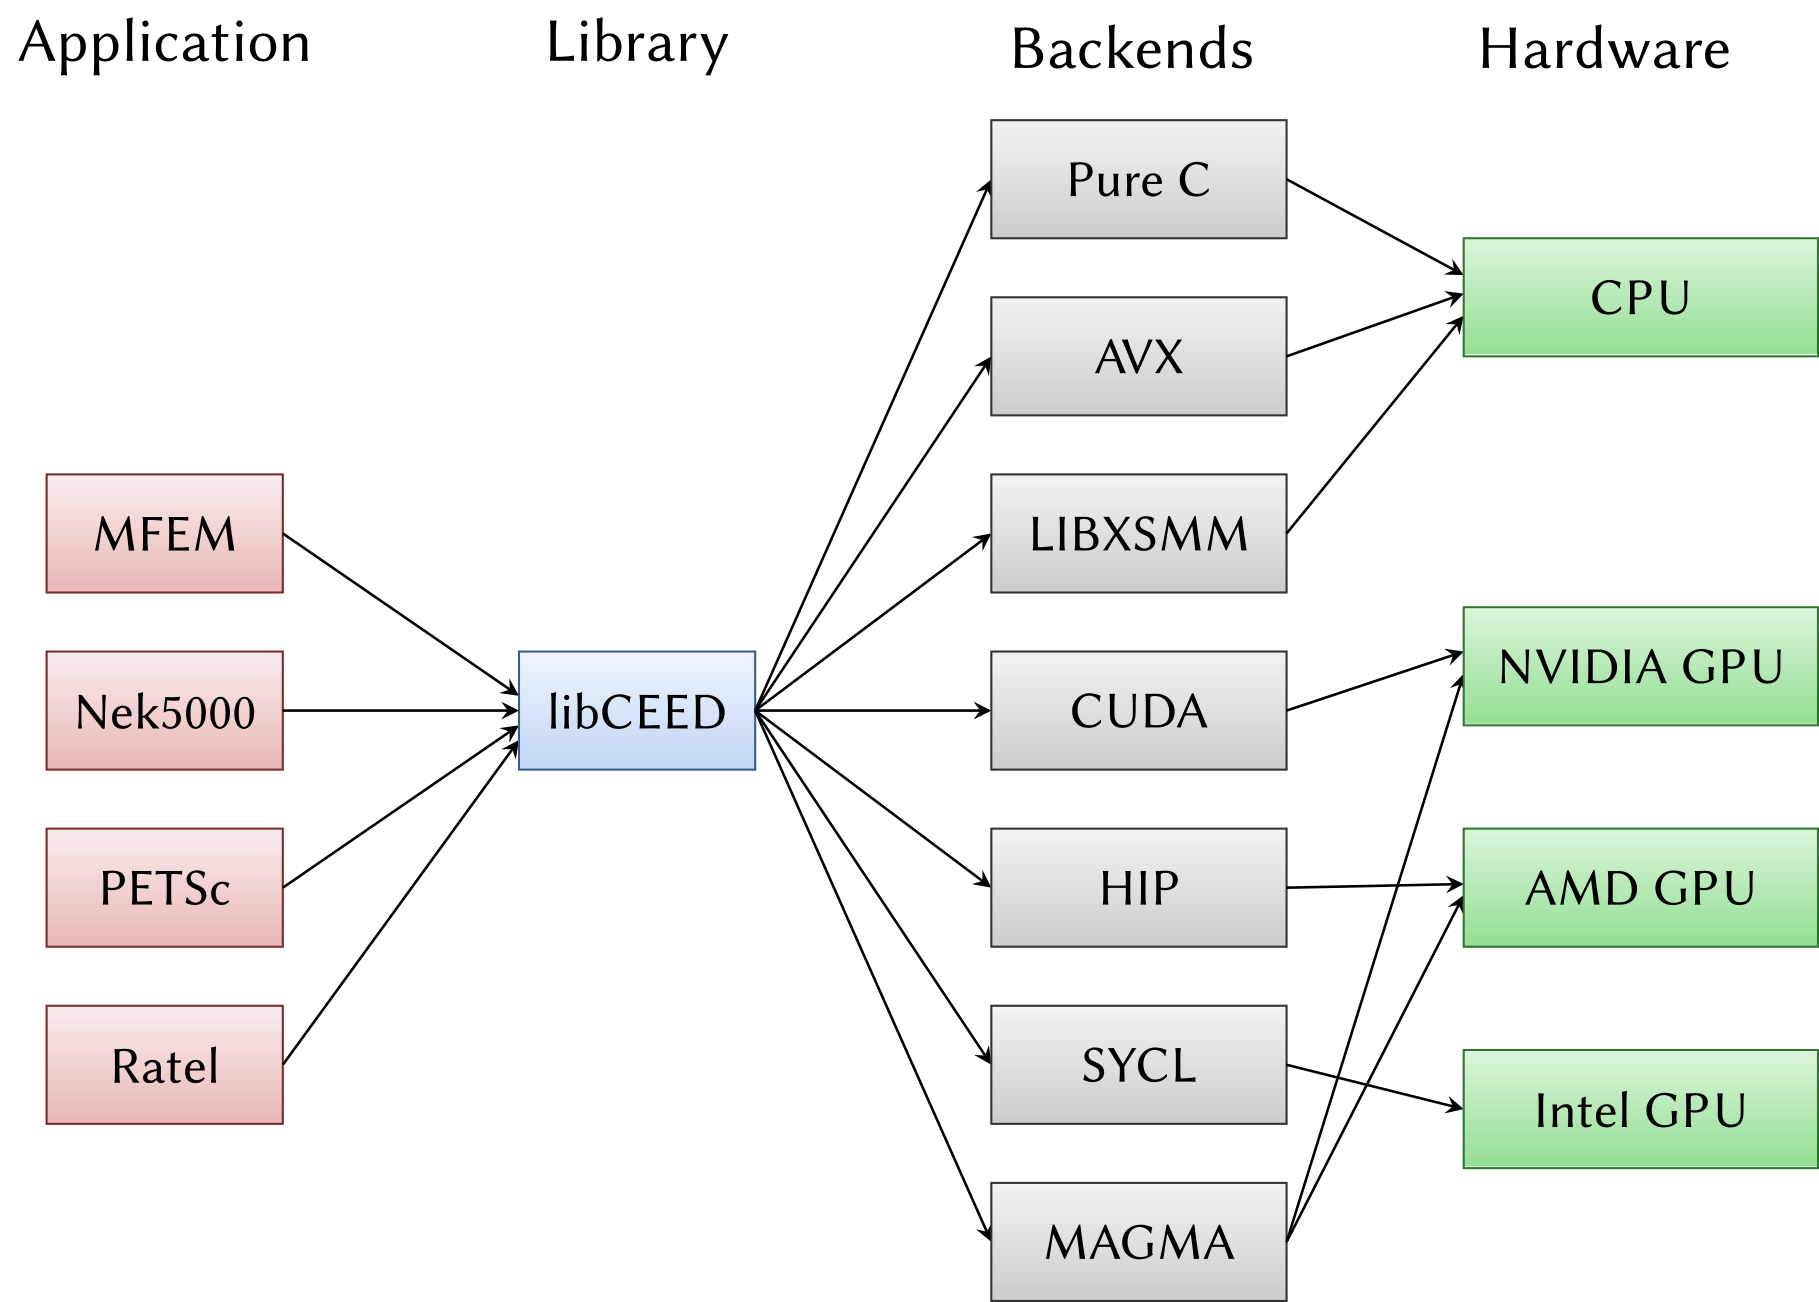
\includegraphics[height=6.5cm]{libCEEDBackends}\\

Natural use case for bridge pattern\\

\end{center}
\end{frame}

%------------------------------------------------

\begin{frame}
\begin{center}
\frametitle{libCEED Operator Decomposition}

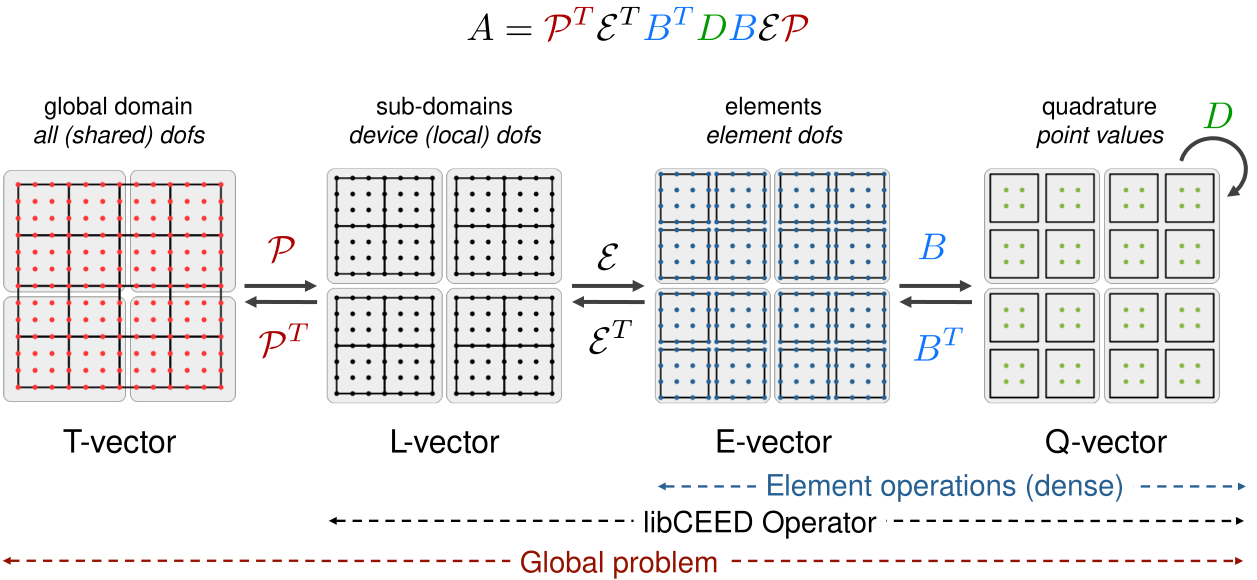
\includegraphics[height=4.5cm]{libCEEDAPI}

\small{

\hspace{1.8cm}${\color{burgundy}A}_L = G^T {\color{blue(ncs)}B^T} {\color{applegreen}D} {\color{blue(ncs)}B} G$

\begin{itemize}

\item $G$ - CeedElemRestriction, local gather/scatter

\item {\color{blue(ncs)}$B$} - CeedBasis, provides basis operations such as interp and grad

\item {\color{applegreen}$D$} - CeedQFunction, representation of PDE at quadrature points

\item ${\color{burgundy}A}_L$ - CeedOperator, aggregation of Ceed objects for local action of operator

\end{itemize}

}

\end{center}
\end{frame}

%------------------------------------------------

\begin{frame}[fragile]
\begin{center}
\frametitle{User QFunction Source}

User QFunction Code:
{\tiny
\begin{lstlisting}[style=C]
// ---- Fuvisc
const CeedInt Fuviscidx[3][3] = {{0, 1, 2}, {1, 3, 4}, {2, 4, 5}};
for (CeedInt j=0; j<3; j++)
  for (CeedInt k=0; k<3; k++)
    dv[k][j+1][i] -= wJ*(Fu[Fuviscidx[j][0]]*dXdxdXdxT[k][0] +
                         Fu[Fuviscidx[j][1]]*dXdxdXdxT[k][1] +
                         Fu[Fuviscidx[j][2]]*dXdxdXdxT[k][2]);
\end{lstlisting}
}

~\\

Compiled Assembly:
{\tiny
\begin{lstlisting}[style=assembly]
    dv[k][j+1][i] -= wJ*(Fu[Fuviscidx[j][0]]*dXdxdXdxT[k][0] +
b08d:	c5 7d 28 d0          	vmovapd %ymm0,%ymm10
                         Fu[Fuviscidx[j][1]]*dXdxdXdxT[k][1] +
b091:	c4 42 c5 b8 d3       	vfmadd231pd %ymm11,%ymm7,%ymm10
b096:	c5 fd 28 84 24 c8 04 	vmovapd 0x4c8(%rsp),%ymm0
b09d:	00 00 
    dv[k][j+1][i] -= wJ*(Fu[Fuviscidx[j][0]]*dXdxdXdxT[k][0] +
b09f:	c4 62 f5 ac 14 07    	vfnmadd213pd (%rdi,%rax,1),%ymm1,%ymm10
b0a5:	c5 7d 11 14 07       	vmovupd %ymm10,(%rdi,%rax,1)
                         Fu[Fuviscidx[j][1]]*dXdxdXdxT[k][1] +
b0aa:	c5 7d 59 94 24 68 04 	vmulpd 0x468(%rsp),%ymm0,%ymm10
b0b1:	00 00
\end{lstlisting}
}

~\\

Similar optimized code on other architectures

\end{center}
\end{frame}

%------------------------------------------------
\section{Backend Development}
%------------------------------------------------

\begin{frame}
\begin{center}
\frametitle{End Goal: Optimized Backends}

CPU:\\

\begin{itemize}

\item AVX instructions for vector operations, FMA\\

~\\

\item LIBXSMM for JiT optimized small matrix multiplication\\

\end{itemize}\\

~\\

~\\

GPU:\\

\begin{itemize}

\item JiT to generate device kernels from user code\\

~\\

\item Fused kernels to minimize launches and data movement\\

\end{itemize}

\end{center}
\end{frame}

%------------------------------------------------

\begin{frame}
\begin{center}
\frametitle{Development Challenges}

CPU:\\

\begin{itemize}

\item Optimized code can be difficult to read\\

~\\

\item External library calls can be opaque\\

\end{itemize}\\

~\\

~\\

GPU:\\

\begin{itemize}

\item Debugging more challenging on devices\\

~\\

\item Fused kernels can't be incrementally tested\\

\end{itemize}

\end{center}
\end{frame}

%------------------------------------------------

\begin{frame}
\begin{center}
\frametitle{Bridge Pattern FTW}

Strong encapsulation of backend implementation details from interface\\

~\\

\begin{itemize}

\item Reference backends provide straightforward implementation\\

\begin{itemize}

\item \lstinline{/cpu/self/ref/serial}

\item \lstinline{/gpu/cuda/ref}

\item \lstinline{/gpu/hip/ref}

\end{itemize}

~\\

\item Debugging backends provide additional debugging tools\\

\begin{itemize}

\item \lstinline{/cpu/self/memcheck}

\end{itemize}

~\\

\item Optimized backends selectively re-implement objects\\

\begin{itemize}

\item \lstinline{/cpu/self/xsmm/blocked}

\item \lstinline{/gpu/cuda/gen}

\end{itemize}

\end{itemize}

\end{center}
\end{frame}

%------------------------------------------------

\begin{frame}
\begin{center}
\frametitle{Hidden Benefits}

\begin{itemize}

\item Stable API and ABI across implementations\\

~\\

\item Flexible and distributed development\\

~\\

\item Clear reference code for new developers\\

~\\

\item Improved debugability ,for users and developers\\

~\\

\item ...

\end{itemize}

\end{center}
\end{frame}

%------------------------------------------------
\section{Future Work}
%------------------------------------------------

\begin{frame}
\begin{center}
\frametitle{Future Work}

\begin{itemize}

\item Further performance enhancements (GPU and CPU)\\

~\\

\item Improved mixed mesh and operator composition support\\

~\\

\item Expanded non-linear and multi-physics examples\\

~\\

\item Preconditioning based on libCEED operator decomposition\\

~\\

\item Algorithmic differentiation of user quadrature functions\\

~\\

\item We invite contributors and friendly users

\end{itemize}

\end{center}
\end{frame}

%------------------------------------------------
\section{Questions}
%------------------------------------------------

\begin{frame}
\begin{center}
\frametitle{Questions?}

{\flushleft

Advisors : \hspace{5mm} Jed Brown\textsuperscript{1} \& Adriana Gillman\textsuperscript{1}\\

~\\

Developers: \hspace{2mm} Ahmad Abdelfattah\textsuperscript{1},
Valeria Barra\textsuperscript{2},\\
Natalie Beams\textsuperscript{1},
Jed Brown\textsuperscript{2},
Jean-Sylvain Camier\textsuperscript{3},\\
Veselin Dobrev\textsuperscript{3},
Yohann Dudouit\textsuperscript{3},
Leila Ghaffari\textsuperscript{2},\\
Tzanio Kolev\textsuperscript{3},
David Medina\textsuperscript{4},
Thilina Rathnayake\textsuperscript{5},\\
\&
Stan Tomov\textsuperscript{5}\\

~\\

Grant: \hspace{11mm} Exascale Computing Project (17-SC-20-SC)\\

~\\

~\\

\small{1: University of Tennesse\\
2: University of Colorado, Boulder\\
3: Lawrence Livermore National Laboratory\\
4: Occalytics LLC\\
5: University of Illinois at Urbana-Champaign\\}}

\end{center}
\end{frame}

%------------------------------------------------

\begin{frame}[noframenumbering]
\titlepage % Print the title page
\end{frame}

%------------------------------------------------

%----------------------------------------------------------------------------------------

\end{document}

